\documentclass[12pt]{report}
\usepackage{amsmath}
\usepackage{mathrsfs}
\usepackage{amssymb}
\usepackage{amsfonts}
\usepackage{gauss}
\usepackage[top=1in,bottom=1in,left=1in,right=1in]{geometry}
\usepackage{dsfont}
\usepackage{amsthm}
\usepackage{graphicx}
\usepackage{multirow}
\usepackage{accents}
\usepackage{statex}
\usepackage{titlepic}
\usepackage{fancyhdr}
\usepackage{tocloft}
\usepackage{multirow}

\usepackage{listings}
\lstset{language=c++}

\usepackage{color}
\usepackage{xcolor}
\definecolor{haizakura}{HTML}{D7C4BB}
\definecolor{mizugaki}{HTML}{B9887D}

\pagestyle{fancy}
\renewcommand{\footrulewidth}{1pt}
\cfoot{ }
\rfoot{\bfseries Fan\ \thepage}

\begin{document}
\begin{titlepage}

\center

\vfill
\includegraphics[height=4cm]{kth_logo.png}\\[0.5cm]

\rule{\linewidth}{0.2mm} \\[4cm]

\textsc{\Large XML for Publishing \\ dm2517}\\[3cm]

\textsc{\Large Project Report}\\[5cm]



\centering \Large \textsc{Fan Yiming} \\
\normalsize \texttt{yimingf@kth.se} \\[0.5cm]
%\normalsize \textsc{In collaboration with}\\[0.5cm]
%\Large \textsc{Xu, Shuqi}\\
%\normalsize \texttt{5123709169}
\vfill

\end{titlepage}

\section*{1 Introduction}
Pok�mon (aka pocket monsters) is a media franchise started by the Pok�mon
Company in Japan in 1995. The world is centered with fictional creatures called ?Pok�mon?. In this world, people could encounter, capture and collect various kinds of Pok�mons. Moreover, Pok�mons could fight each other for their masters. Started in 1990s, the Pok�mon quickly became a hit throughout Japan and the rest of the world. The animations, comic and games of Pok�mon were successfully sold in the pasting 20 years. By now, there are 26 generations of Pok�mon video games with totally 720 different Pok�mons released.\newline
Collecting Pok�mons is an interesting but tedious job. Some Pok�mons have extremely criticaly requirement to be captured, which increases the difficulty of obtaining a whole collection of Pok�mons. Therefore, to create an online ``capturing handbook'' for those Pok�mon-holics becomes important. This project is aimed at visualizing a database for all those Pok�mons with adequate informations, both for fans and free-lookers.

\section*{2 The use of the system}
Fortunately the system is designed with a pretty simple interface. The index page look like shown below, and the user could fetch some of the pokemons on the main page.
\begin{center} 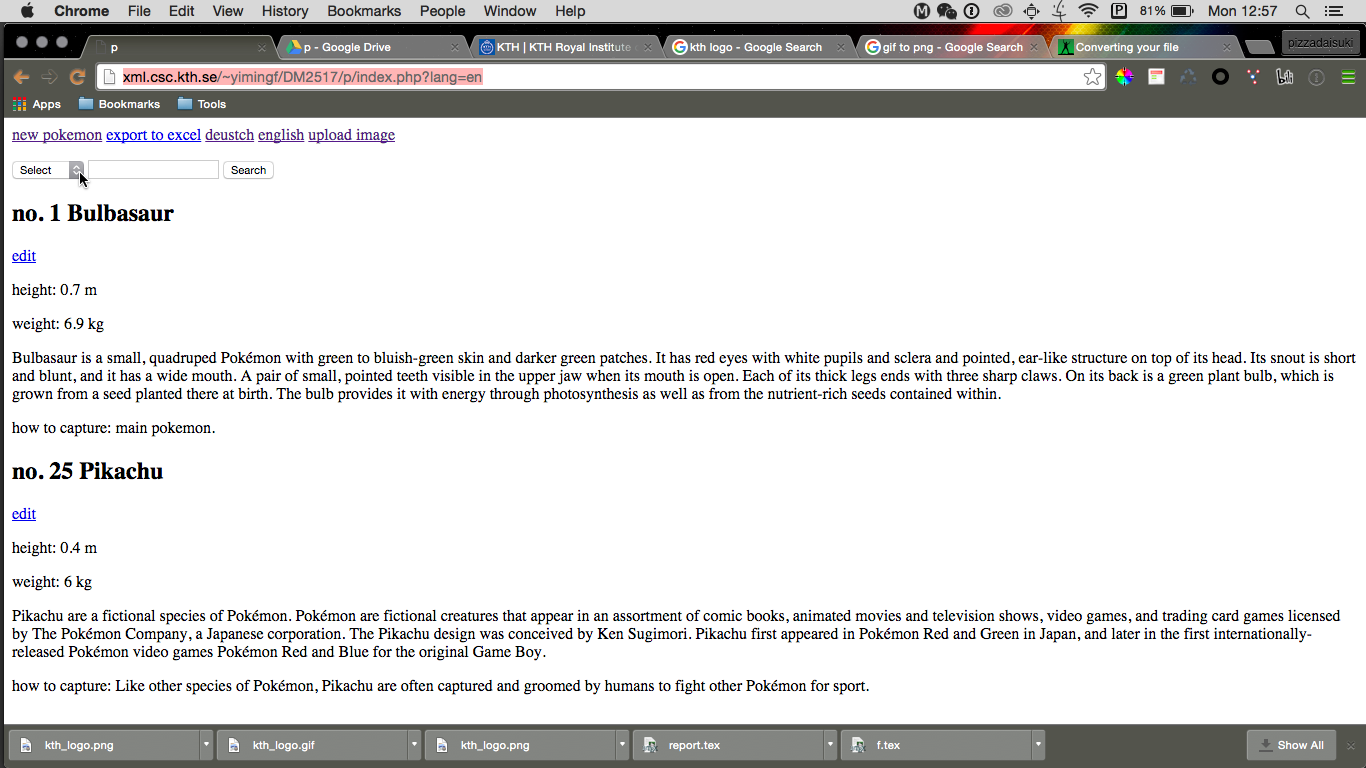
\includegraphics[width=16cm]{2_1.png} \end{center}
As shown on the screenshot, by scrolling up and down the screen, the user could get the information of the pokemons. The characteristics include:
\begin{itemize}
\item the name
\item the height of the pokemon,
\item the weight of the pokemon,
\item the brief introduction and
\item the basic method for capturing the pokemon
\end{itemize}
Due the the limit of due time of the project, some detailed information of pokemons were not implemented yet.\newline
When the user intend to edit the characteristics of one certain pokemon, he/she could click the `edit' button below the name of the selected pokemon. After clicking, the edit interface is shown.
\begin{center}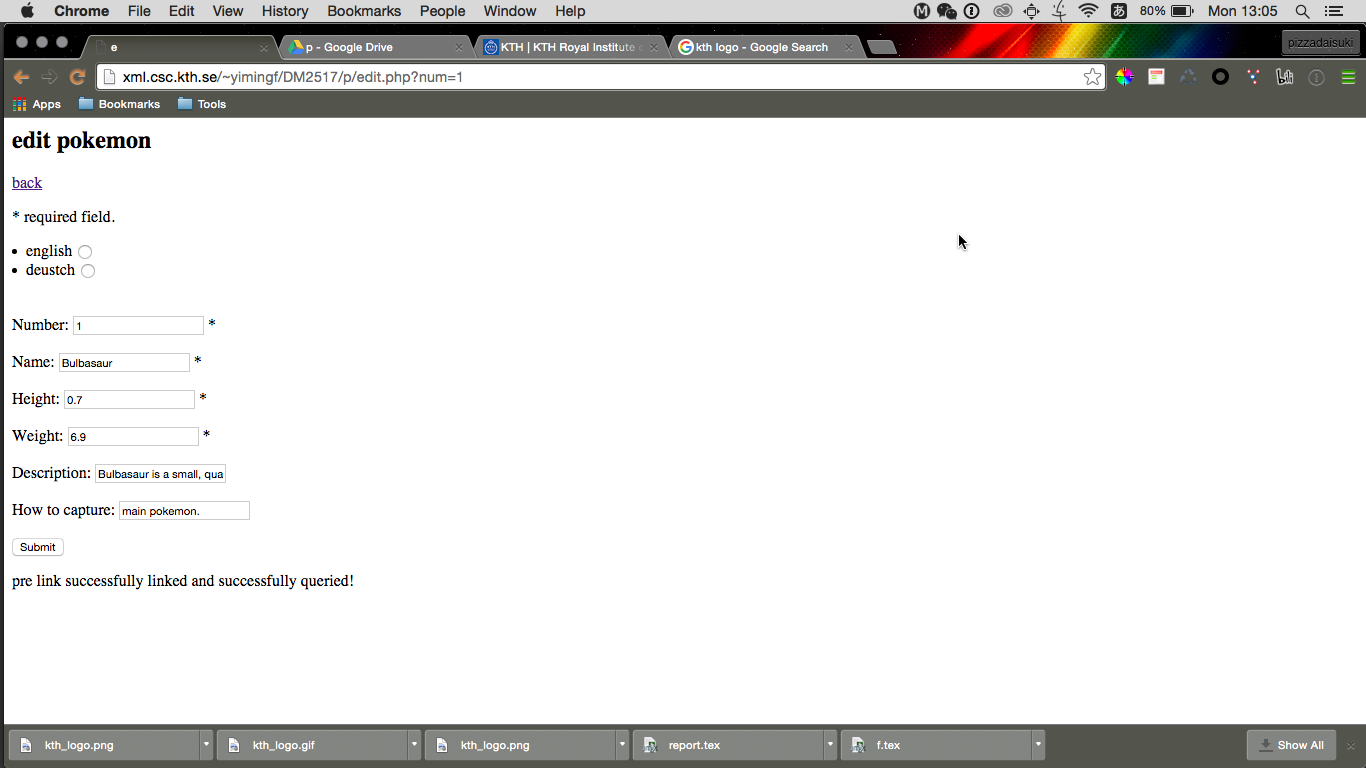
\includegraphics[width=16cm]{2_2.png}\end{center}
As shown on the screenshot, the pre-existing information of the pokemon has been fetched out onto the edit labels. After editing, the user could submit them. Then a message would be prompted, if the editing action succeeds.\newline
After editing the user would be directed back to the index page.\newline
The user is also allowed to add new pokemons. By clicking the `new pokemon' button on the top of the index page, the user could be directed to an edit page.
\begin{center} 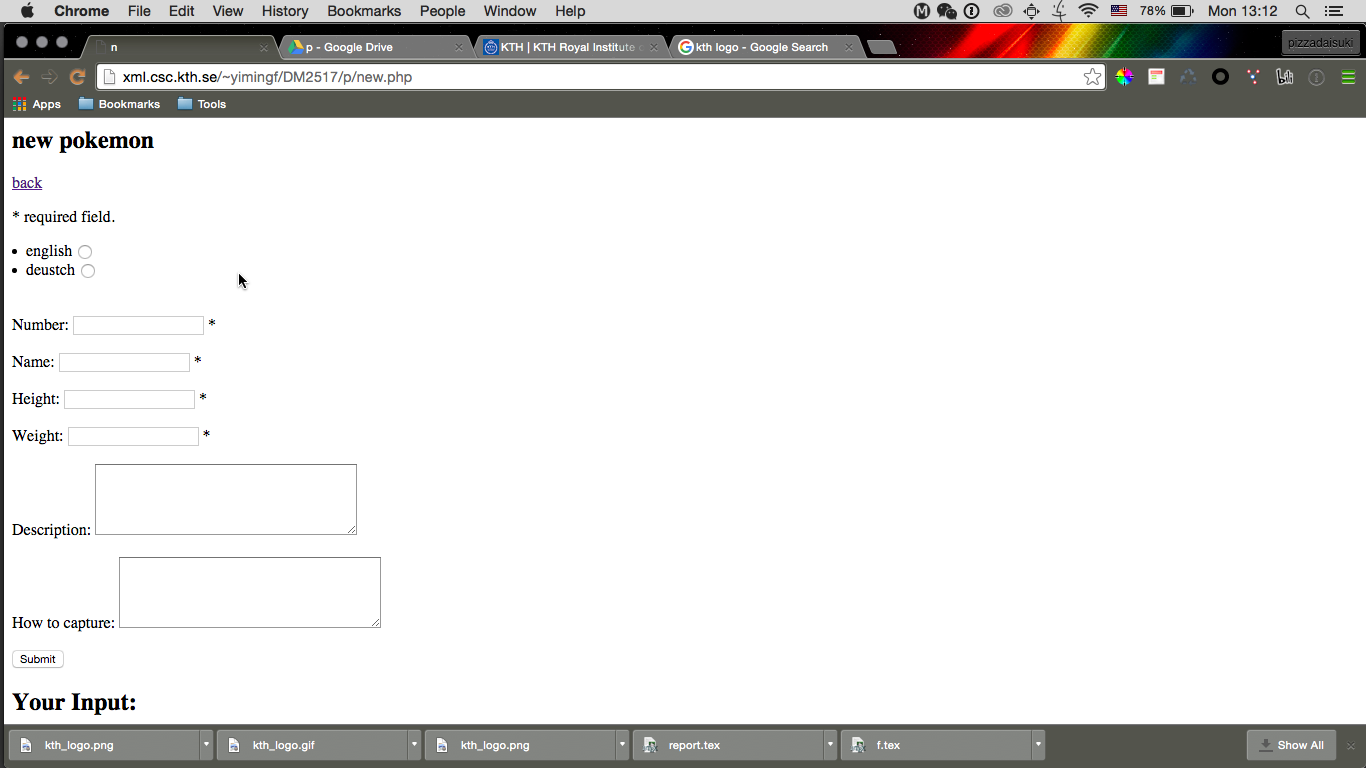
\includegraphics[width=16cm]{2_3.png} \end{center}
notice that the user are always allowed to specify the language he/she is using when adding and editing the pokemon. This is what we called the `multi-language' function integrated in the whole system. Due to the time limit the user are only allowed to select language between English and Deutsch.\newline
When all legal information is written inside the label, the user could click the `submit' button to submit the information to the database. Then the user would receive a message indicating if the operation is successful.\newline
When the insertion is done the user could press the `back' button to see what has changed in the index page.
\begin{center} 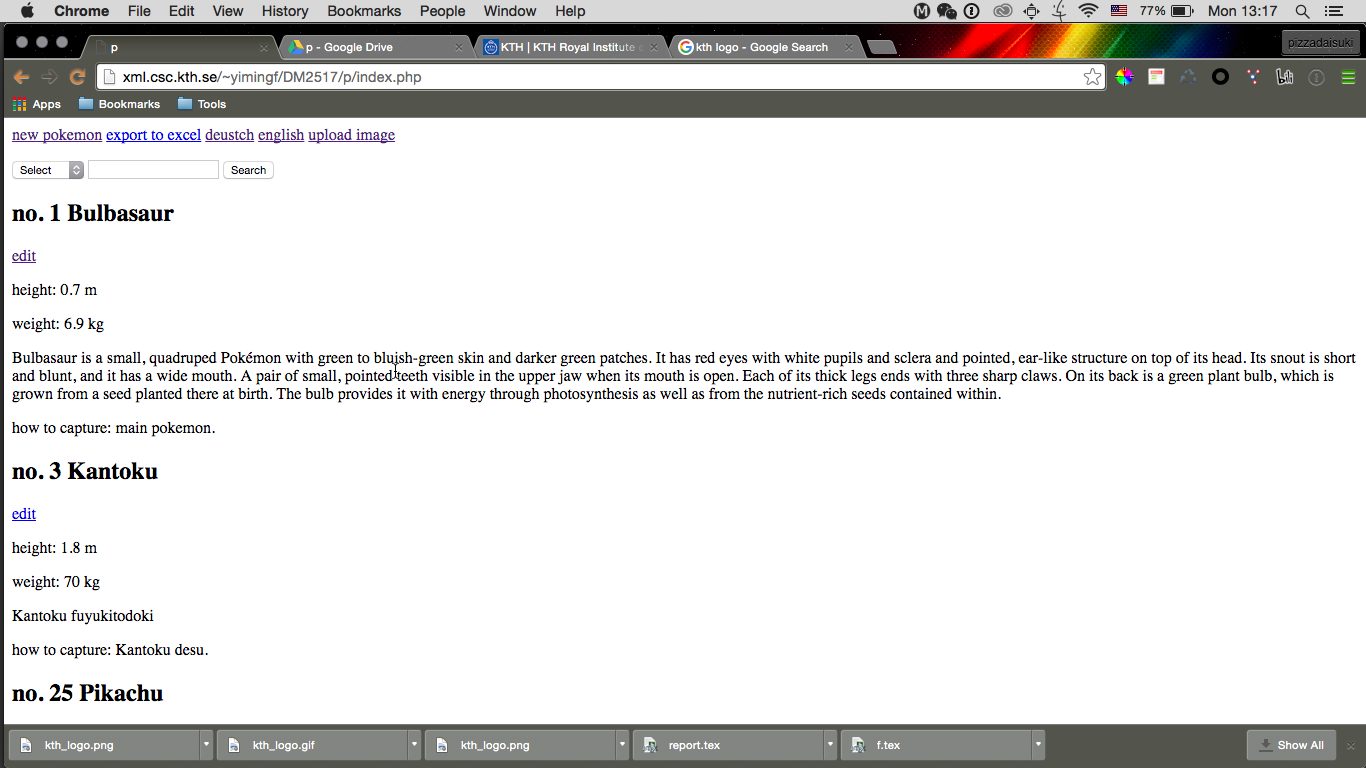
\includegraphics[width=16cm]{2_4.png} \end{center}
Now the virtual `pokemon' called \textit{Kantoku} was successfully inserted.\newline
As is said above, the system also supports multi-language function. By pressing the `Deutsch' or `English' button, the user could switch the language he/she wants to see. The Deutsch interface is shown below.
\begin{center} 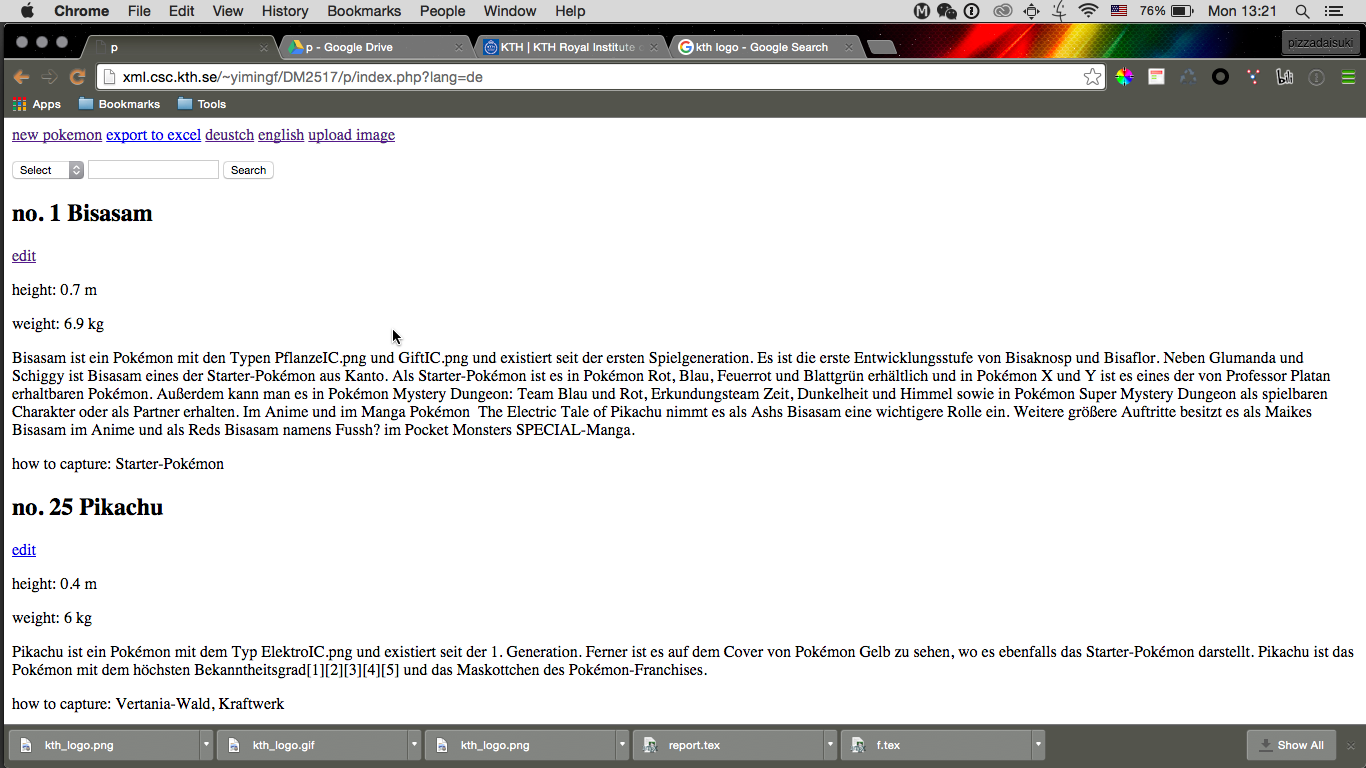
\includegraphics[width=16cm]{2_5.png} \end{center}
Notice that we have just added a virtual pokemon called \textit{Kantoku}. Since we have only added the English characteristics of this pokemon, we are not able to see its Deutsch characteristics now.\newline
The system also supports `exporting to excel' function for multi-tube publishing. By clicking the `export to excel' button on the top of the index page, the user could download the information of all pokemons with the format of \textit{xls}.
\begin{center} 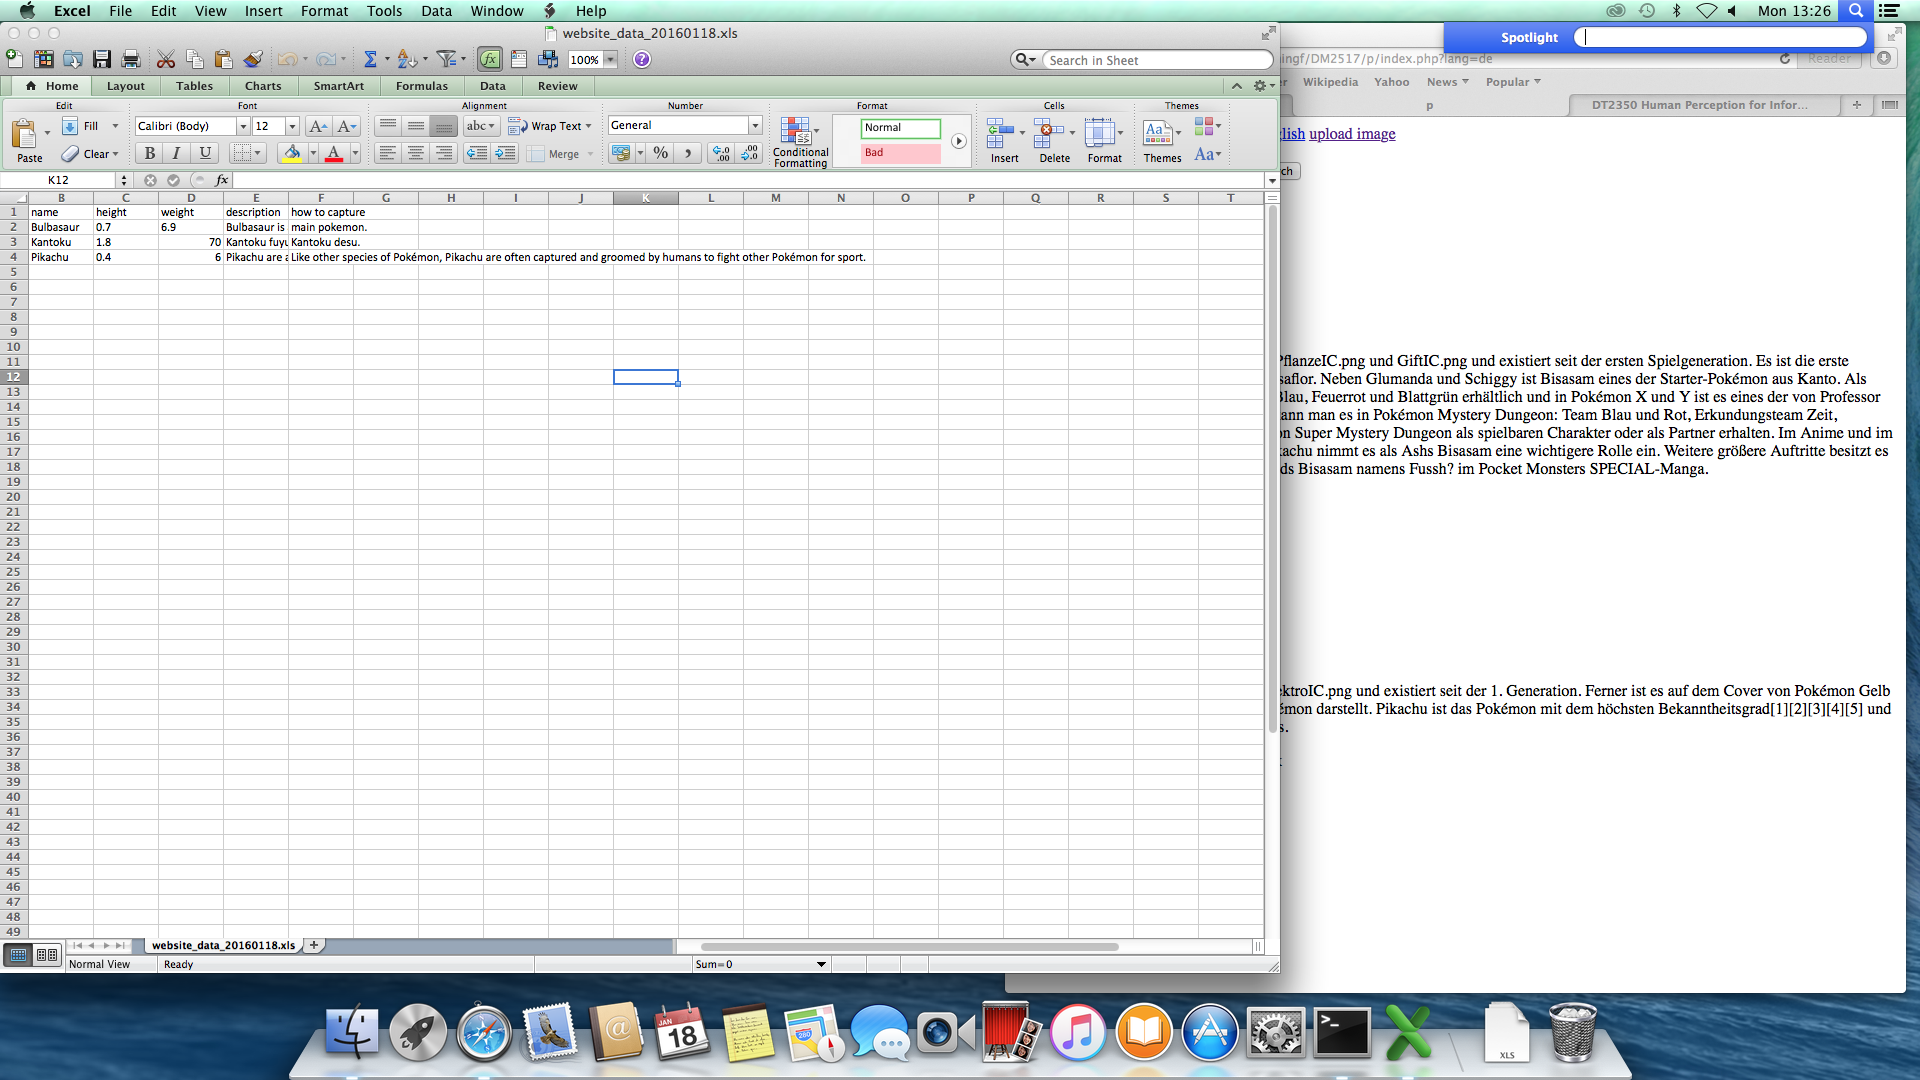
\includegraphics[width=16cm]{2_6.png} \end{center}
As shown above, all the information of the pokemons are stored in the \textit{xls} file.\newline
The system also supports searching function. By select the \textit{category} and the specification on the top of the index page, the user could select the pokemon with intended characteristics. Below shows the result with specification `index = 1':
\begin{center} 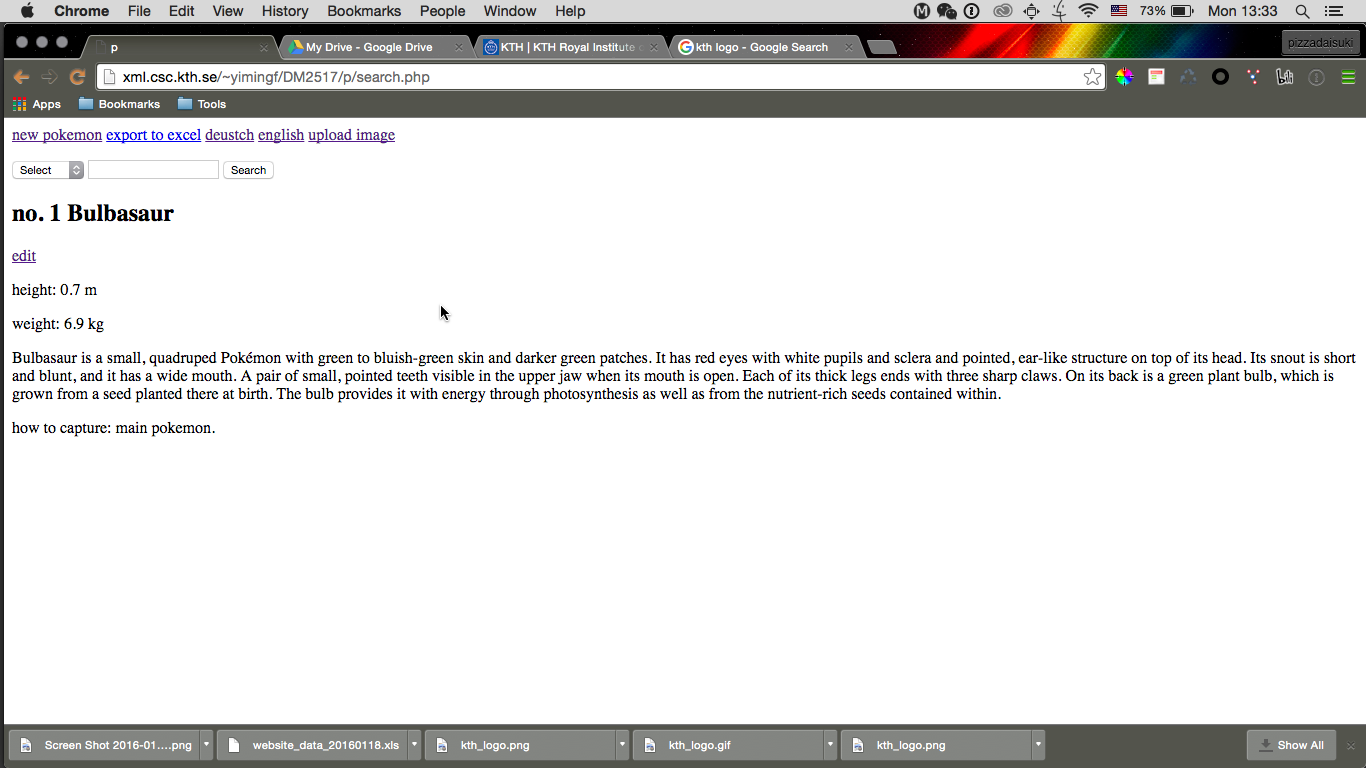
\includegraphics[width=16cm]{2_7.png} \end{center}

\section*{3 Reflection}
This project is done, but some of the features are not implemented, due to the time limit of the project. These missing features (comparing to my initial proposal of the project) are:
\begin{itemize}
\item Japanese language support
\item more characteristics of the pokemon
\item more vivid interface
\item multi-user support, and so on.
\end{itemize}
Anyway I consider this project simple but complete. All basic functions plus some extra functions are implemented correctly. I consider this project a good chance for me to combine the knowledge of XML and web programming.

\end{document}